\documentclass{standalone}
\usepackage{tikz}
\usetikzlibrary{patterns}
\usetikzlibrary{positioning}
\usetikzlibrary{patterns, positioning}
\usetikzlibrary{shapes.misc}
\usepackage[outline]{contour}
\contourlength{1.5pt} 


\begin{document}
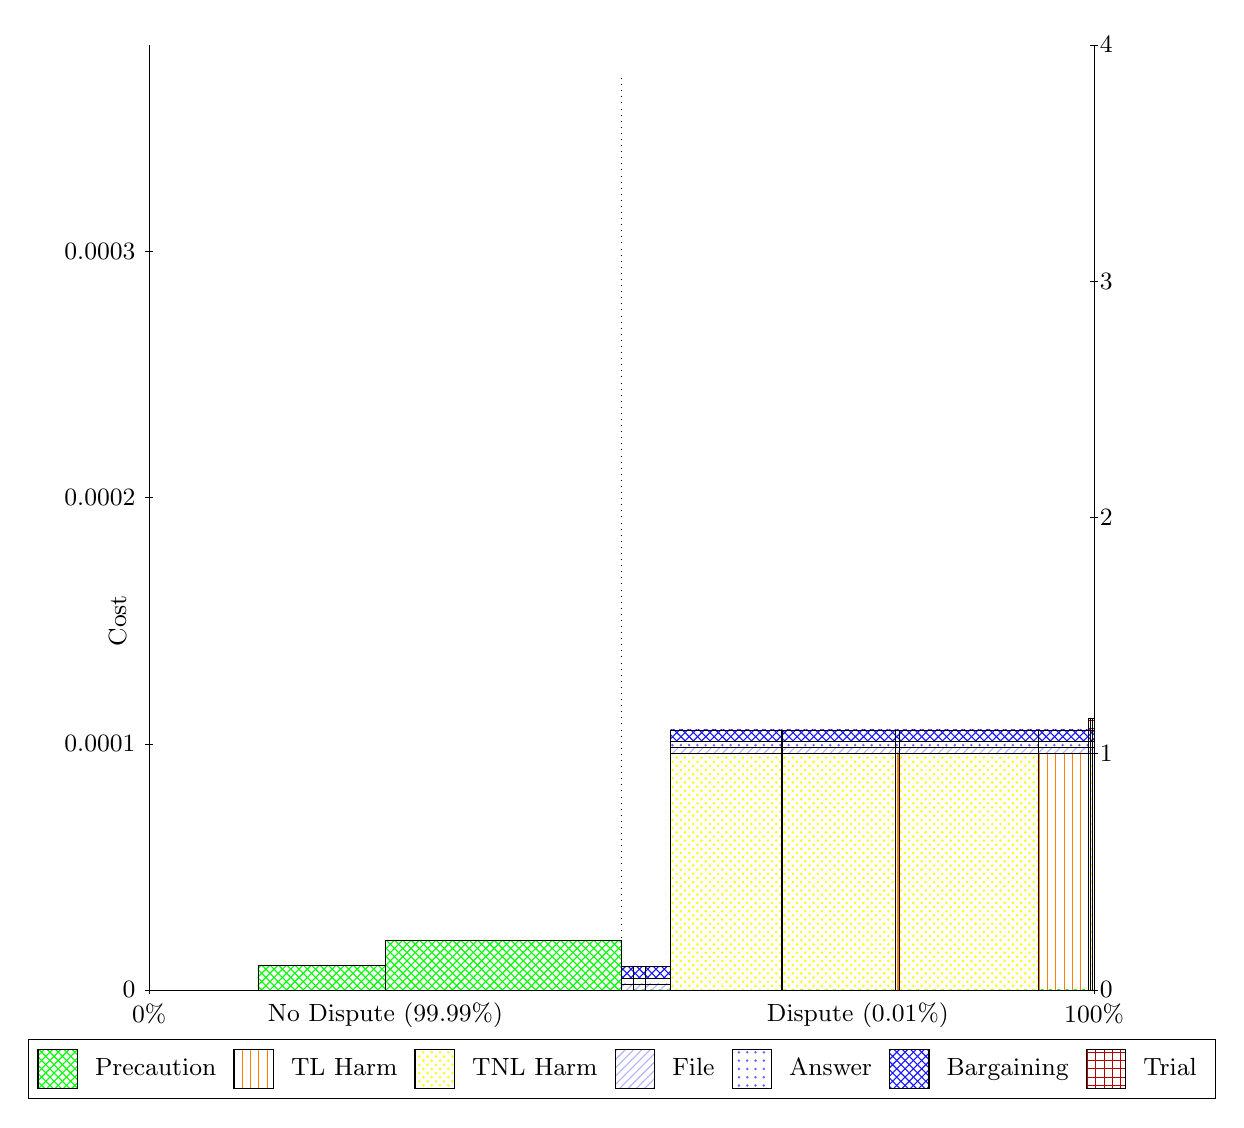
\begin{tikzpicture}
\draw[pattern=crosshatch, pattern color=green,draw=black,very thin] (2.8801,2.5) rectangle (4.5,2.8124);
\draw[pattern=crosshatch, pattern color=green,draw=black,very thin] (4.5,2.5) rectangle (7.5,3.1249);
\draw[pattern=north east lines, pattern color=blue!30,draw=black,very thin] (7.5,2.5) rectangle (7.6412,2.575);
\draw[pattern=dots,  pattern color=blue!60,draw=black,very thin] (7.5,2.575) rectangle (7.6412,2.65);
\draw[pattern=crosshatch,      pattern color=blue!90,draw=black,very thin] (7.5,2.65) rectangle (7.6412,2.8);
\draw[pattern=crosshatch, pattern color=green,draw=black,very thin] (7.6412,2.5) rectangle (7.8046,2.5);
\draw[pattern=north east lines, pattern color=blue!30,draw=black,very thin] (7.6412,2.5) rectangle (7.8046,2.575);
\draw[pattern=dots,  pattern color=blue!60,draw=black,very thin] (7.6412,2.575) rectangle (7.8046,2.65);
\draw[pattern=crosshatch,      pattern color=blue!90,draw=black,very thin] (7.6412,2.65) rectangle (7.8046,2.8);
\draw[pattern=crosshatch, pattern color=green,draw=black,very thin] (7.8046,2.5) rectangle (8.117,2.5001);
\draw[pattern=north east lines, pattern color=blue!30,draw=black,very thin] (7.8046,2.5001) rectangle (8.117,2.5751);
\draw[pattern=dots,  pattern color=blue!60,draw=black,very thin] (7.8046,2.5751) rectangle (8.117,2.6501);
\draw[pattern=crosshatch,      pattern color=blue!90,draw=black,very thin] (7.8046,2.6501) rectangle (8.117,2.8001);
\draw[pattern=crosshatch, pattern color=green,draw=black,very thin] (8.117,2.5) rectangle (8.1223,2.5);
\draw[pattern=north east lines, pattern color=blue!30,draw=black,very thin] (8.117,2.5) rectangle (8.1223,2.575);
\draw[pattern=dots,  pattern color=blue!60,draw=black,very thin] (8.117,2.575) rectangle (8.1223,2.65);
\draw[pattern=crosshatch,      pattern color=blue!90,draw=black,very thin] (8.117,2.65) rectangle (8.1223,2.8);
\draw[pattern=grid,            pattern color=red!70!black,draw=black,very thin] (8.117,2.8) rectangle (8.1223,2.95);
\draw[pattern=crosshatch dots, pattern color=yellow,draw=black,very thin] (8.1223,2.5) rectangle (9.5268,5.5);
\draw[pattern=north east lines, pattern color=blue!30,draw=black,very thin] (8.1223,5.5) rectangle (9.5268,5.575);
\draw[pattern=dots,  pattern color=blue!60,draw=black,very thin] (8.1223,5.575) rectangle (9.5268,5.65);
\draw[pattern=crosshatch,      pattern color=blue!90,draw=black,very thin] (8.1223,5.65) rectangle (9.5268,5.8);
\draw[pattern=vertical lines, pattern color=orange,draw=black,very thin] (9.5268,2.5) rectangle (9.5342,5.5);
\draw[pattern=north east lines, pattern color=blue!30,draw=black,very thin] (9.5268,5.5) rectangle (9.5342,5.575);
\draw[pattern=dots,  pattern color=blue!60,draw=black,very thin] (9.5268,5.575) rectangle (9.5342,5.65);
\draw[pattern=crosshatch,      pattern color=blue!90,draw=black,very thin] (9.5268,5.65) rectangle (9.5342,5.8);
\draw[pattern=crosshatch, pattern color=green,draw=black,very thin] (9.5342,2.5) rectangle (10.974,2.5);
\draw[pattern=crosshatch dots, pattern color=yellow,draw=black,very thin] (9.5342,2.5) rectangle (10.974,5.5);
\draw[pattern=north east lines, pattern color=blue!30,draw=black,very thin] (9.5342,5.5) rectangle (10.974,5.575);
\draw[pattern=dots,  pattern color=blue!60,draw=black,very thin] (9.5342,5.575) rectangle (10.974,5.65);
\draw[pattern=crosshatch,      pattern color=blue!90,draw=black,very thin] (9.5342,5.65) rectangle (10.974,5.8);
\draw[pattern=crosshatch, pattern color=green,draw=black,very thin] (10.974,2.5) rectangle (11.02,2.5);
\draw[pattern=vertical lines, pattern color=orange,draw=black,very thin] (10.974,2.5) rectangle (11.02,5.5);
\draw[pattern=north east lines, pattern color=blue!30,draw=black,very thin] (10.974,5.5) rectangle (11.02,5.575);
\draw[pattern=dots,  pattern color=blue!60,draw=black,very thin] (10.974,5.575) rectangle (11.02,5.65);
\draw[pattern=crosshatch,      pattern color=blue!90,draw=black,very thin] (10.974,5.65) rectangle (11.02,5.8);
\draw[pattern=crosshatch, pattern color=green,draw=black,very thin] (11.02,2.5) rectangle (12.797,2.5001);
\draw[pattern=crosshatch dots, pattern color=yellow,draw=black,very thin] (11.02,2.5001) rectangle (12.797,5.5001);
\draw[pattern=north east lines, pattern color=blue!30,draw=black,very thin] (11.02,5.5001) rectangle (12.797,5.5751);
\draw[pattern=dots,  pattern color=blue!60,draw=black,very thin] (11.02,5.5751) rectangle (12.797,5.6501);
\draw[pattern=crosshatch,      pattern color=blue!90,draw=black,very thin] (11.02,5.6501) rectangle (12.797,5.8001);
\draw[pattern=crosshatch, pattern color=green,draw=black,very thin] (12.797,2.5) rectangle (13.428,2.5001);
\draw[pattern=vertical lines, pattern color=orange,draw=black,very thin] (12.797,2.5001) rectangle (13.428,5.5001);
\draw[pattern=north east lines, pattern color=blue!30,draw=black,very thin] (12.797,5.5001) rectangle (13.428,5.5751);
\draw[pattern=dots,  pattern color=blue!60,draw=black,very thin] (12.797,5.5751) rectangle (13.428,5.6501);
\draw[pattern=crosshatch,      pattern color=blue!90,draw=black,very thin] (12.797,5.6501) rectangle (13.428,5.8001);
\draw[pattern=crosshatch dots, pattern color=yellow,draw=black,very thin] (13.428,2.5) rectangle (13.448,5.5);
\draw[pattern=north east lines, pattern color=blue!30,draw=black,very thin] (13.428,5.5) rectangle (13.448,5.575);
\draw[pattern=dots,  pattern color=blue!60,draw=black,very thin] (13.428,5.575) rectangle (13.448,5.65);
\draw[pattern=crosshatch,      pattern color=blue!90,draw=black,very thin] (13.428,5.65) rectangle (13.448,5.8);
\draw[pattern=grid,            pattern color=red!70!black,draw=black,very thin] (13.428,5.8) rectangle (13.448,5.95);
\draw[pattern=vertical lines, pattern color=orange,draw=black,very thin] (13.448,2.5) rectangle (13.453,5.5);
\draw[pattern=north east lines, pattern color=blue!30,draw=black,very thin] (13.448,5.5) rectangle (13.453,5.575);
\draw[pattern=dots,  pattern color=blue!60,draw=black,very thin] (13.448,5.575) rectangle (13.453,5.65);
\draw[pattern=crosshatch,      pattern color=blue!90,draw=black,very thin] (13.448,5.65) rectangle (13.453,5.8);
\draw[pattern=grid,            pattern color=red!70!black,draw=black,very thin] (13.448,5.8) rectangle (13.453,5.95);
\draw[pattern=crosshatch, pattern color=green,draw=black,very thin] (13.453,2.5) rectangle (13.481,2.5);
\draw[pattern=crosshatch dots, pattern color=yellow,draw=black,very thin] (13.453,2.5) rectangle (13.481,5.5);
\draw[pattern=north east lines, pattern color=blue!30,draw=black,very thin] (13.453,5.5) rectangle (13.481,5.575);
\draw[pattern=dots,  pattern color=blue!60,draw=black,very thin] (13.453,5.575) rectangle (13.481,5.65);
\draw[pattern=crosshatch,      pattern color=blue!90,draw=black,very thin] (13.453,5.65) rectangle (13.481,5.8);
\draw[pattern=grid,            pattern color=red!70!black,draw=black,very thin] (13.453,5.8) rectangle (13.481,5.95);
\draw[pattern=crosshatch, pattern color=green,draw=black,very thin] (13.481,2.5) rectangle (13.5,2.5);
\draw[pattern=vertical lines, pattern color=orange,draw=black,very thin] (13.481,2.5) rectangle (13.5,5.5);
\draw[pattern=north east lines, pattern color=blue!30,draw=black,very thin] (13.481,5.5) rectangle (13.5,5.575);
\draw[pattern=dots,  pattern color=blue!60,draw=black,very thin] (13.481,5.575) rectangle (13.5,5.65);
\draw[pattern=crosshatch,      pattern color=blue!90,draw=black,very thin] (13.481,5.65) rectangle (13.5,5.8);
\draw[pattern=grid,            pattern color=red!70!black,draw=black,very thin] (13.481,5.8) rectangle (13.5,5.95);
\draw[black,very thin] (1.5,2.5) -- (1.5,14.5);
\node[font=\small,rotate=90,text=black, anchor=center] at (1.1, 7.1866) {Cost};
\draw[black,very thin] (1.45,2.5) -- (1.55,2.5);
\node[font=\small,text=black, anchor=east] at (1.45, 2.5) {0};
\draw[black,very thin] (1.45,5.6244) -- (1.55,5.6244);
\node[font=\small,text=black, anchor=east] at (1.45, 5.6244) {0.0001};
\draw[black,very thin] (1.45,8.7488) -- (1.55,8.7488);
\node[font=\small,text=black, anchor=east] at (1.45, 8.7488) {0.0002};
\draw[black,very thin] (1.45,11.873) -- (1.55,11.873);
\node[font=\small,text=black, anchor=east] at (1.45, 11.873) {0.0003};

\draw[black,dotted,very thin] (7.5,2.86) -- (7.5,14.14);
\draw[black,very thin] (13.5,2.5) -- (13.5,14.5);
\draw[black,very thin] (13.45,2.5) -- (13.55,2.5);
\node[font=\small,text=black, anchor=west] at (13.45, 2.5) {0};
\draw[black,very thin] (13.45,5.5) -- (13.55,5.5);
\node[font=\small,text=black, anchor=west] at (13.45, 5.5) {1};
\draw[black,very thin] (13.45,8.5) -- (13.55,8.5);
\node[font=\small,text=black, anchor=west] at (13.45, 8.5) {2};
\draw[black,very thin] (13.45,11.5) -- (13.55,11.5);
\node[font=\small,text=black, anchor=west] at (13.45, 11.5) {3};
\draw[black,very thin] (13.45,14.5) -- (13.55,14.5);
\node[font=\small,text=black, anchor=west] at (13.45, 14.5) {4};

\draw[black,very thin] (1.5,2.5) -- (13.5,2.5);
\draw[black,very thin] (1.5,2.45) -- (1.5,2.55);
\node[font=\small,text=black, anchor=north] at (1.5, 2.45) {0\%};
\draw[black,very thin] (13.5,2.45) -- (13.5,2.55);
\node[font=\small,text=black, anchor=north] at (13.5, 2.45) {100\%};

\node[font=\small,text=black,anchor=south] at (4.5, 1.9) {No\ Dispute\ (99.99\%)};
\node[font=\small,text=black,anchor=south] at (10.5, 1.9) {Dispute\ (0.01\%)};
\draw (7.5,2.5) node (B) {};
\begin{scope}[align=center]
\matrix[scale=0.5,draw=black,below=0.5cm of B,nodes={draw},column sep=0.1cm]{
\node[rectangle,draw,minimum width=0.5cm,minimum height=0.5cm,pattern=crosshatch, pattern color=green]{}; & \node[draw=none,font=\small,text=black]{Precaution}; &
\node[rectangle,draw,minimum width=0.5cm,minimum height=0.5cm,pattern=vertical lines, pattern color=orange]{}; & \node[draw=none,font=\small,text=black]{TL Harm}; &
\node[rectangle,draw,minimum width=0.5cm,minimum height=0.5cm,pattern=crosshatch dots, pattern color=yellow]{}; & \node[draw=none,font=\small,text=black]{TNL Harm}; &
\node[rectangle,draw,minimum width=0.5cm,minimum height=0.5cm,pattern=north east lines, pattern color=blue!30]{}; & \node[draw=none,font=\small,text=black]{File}; &
\node[rectangle,draw,minimum width=0.5cm,minimum height=0.5cm,pattern=dots,  pattern color=blue!60]{}; & \node[draw=none,font=\small,text=black]{Answer}; &
\node[rectangle,draw,minimum width=0.5cm,minimum height=0.5cm,pattern=crosshatch,      pattern color=blue!90]{}; & \node[draw=none,font=\small,text=black]{Bargaining}; &
\node[rectangle,draw,minimum width=0.5cm,minimum height=0.5cm,pattern=grid,            pattern color=red!70!black]{}; & \node[draw=none,font=\small,text=black]{Trial}; \\\\
};\end{scope}

\end{tikzpicture}
\end{document}